\documentclass[12pt]{extarticle}
\usepackage[utf8]{inputenc}
\usepackage{graphicx}
\usepackage{float}

% Disable indentation
\setlength{\parindent}{0pt}

\title{Lab 8: Network virtualization with Virtualbox}
\author{Alexander Hoffmann}
\date{\today}

\begin{document}

\maketitle

\section{Configuration}
For this lab, we will configure our virtual machines in a host-only network. Host-only networking can be thought of as a hybrid between the bridged and internal networking modes. As with bridged networking, the virtual machines can talk to each other and the host as if they were connected through a physical Ethernet switch. As with internal networking, a physical networking interface need not be present, and the virtual machines cannot talk to the world outside the host since they are not connected to a physical networking interface.\\

When host-only networking is used, Oracle VM VirtualBox creates a new software interface on the host which then appears next to your existing network interfaces. In other words, whereas with bridged networking an existing physical interface is used to attach virtual machines to, with host-only networking a new loopback interface is created on the host. And whereas with internal networking, the traffic between the virtual machines cannot be seen, the traffic on the loopback interface on the host can be intercepted.\\

\textbf{1.} First, we need to configure the virtual interfaces in the VirtualBox GUI. Here is the current configuration:\\~\\
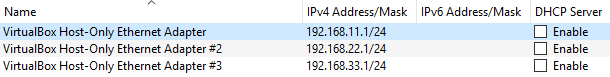
\includegraphics[scale=0.8]{resources/1-1-0.png}\\
These are our three networks. Next, we'll manually configure the IP addresses inside the virtual machines. The command is as follows:
\begin{verbatim}
ifconfig <interface> <ip-address> netmask <netmask> up
\end{verbatim}
Which yields the following results after configuration:\\
\begin{center}
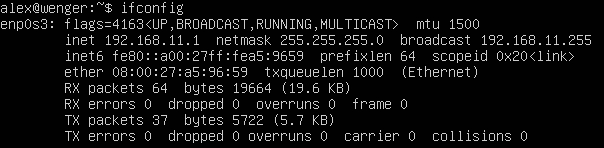
\includegraphics[scale=0.8]{resources/1-1-1.png}\\
PC Router\\~\\
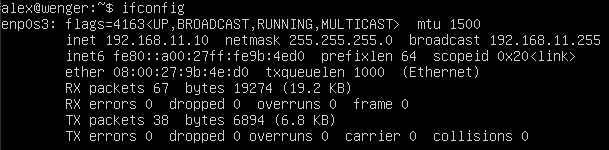
\includegraphics[scale=0.8]{resources/1-1-2.png}\\
PC1\\~\\
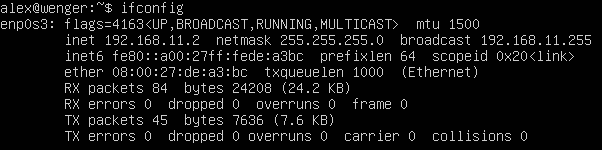
\includegraphics[scale=0.8]{resources/1-1-3.png}\\
Server
\end{center}

The next step is to disconnect the host machine from host-only network 1 and 2.\\
\begin{center}
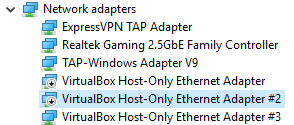
\includegraphics[scale=0.8]{resources/1-0-0.png}\\
\end{center}

\textbf{2.} Now we do the same for the second interface.
\begin{center}
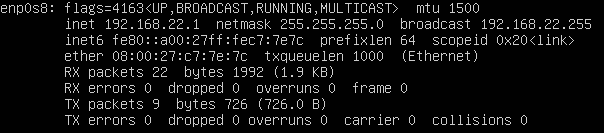
\includegraphics[scale=0.8]{resources/1-2-1.png}\\
PC Router\\~\\
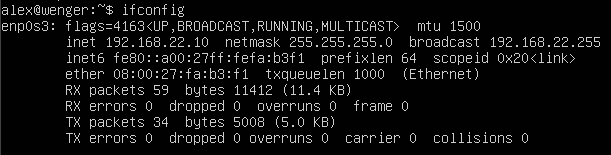
\includegraphics[scale=0.8]{resources/1-2-2.png}\\
PC2
\end{center}

\textbf{3.} Finally, configure the third interface.
\begin{center}
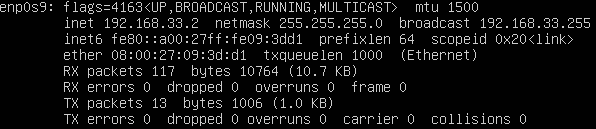
\includegraphics[scale=0.8]{resources/1-3-1.png}\\
PC Router\\~\\
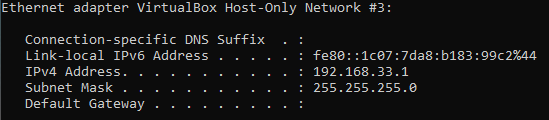
\includegraphics[scale=0.8]{resources/1-3-2.png}\\
PC Host
\end{center}

\section{Testing}
\textbf{1.} Testing pings from various devices.\\
\begin{center}
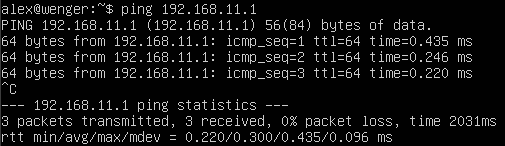
\includegraphics[scale=0.8]{resources/2-1-1.png}\\
Ping PC Router from PC1\\~\\
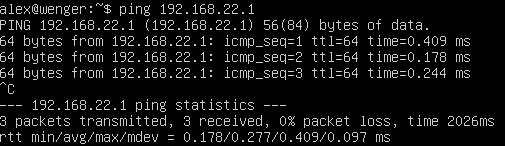
\includegraphics[scale=0.8]{resources/2-1-2.png}\\
Ping PC Router from PC2\\~\\
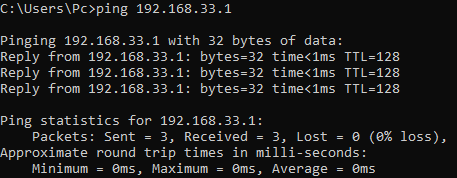
\includegraphics[scale=0.8]{resources/2-1-3.png}\\
Ping PC Router from PC Host\\~\\
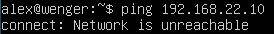
\includegraphics[scale=0.8]{resources/2-1-4.png}\\
Ping PC2 from Server\\~\\
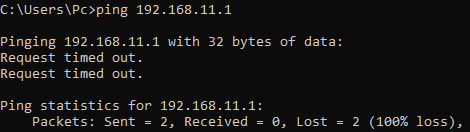
\includegraphics[scale=0.8]{resources/2-1-5.png}\\
Ping PC1 from PC Host
\end{center}

\textbf{2.} There are two pings that have failed:
\begin{itemize}
\item ping from Server to PC2
\item ping from PC Host to PC1
\end{itemize}
Both these pings failed because we tried to access devices on different networks without advertising them in the first place. We need to add gateways in order to allow the devices on different networks to communicate with each other through the router.\\

\textbf{3.} We have to add default gateways on each device so that it forwards unknown traffic. Use this command:
\begin{verbatim}
route add default gw <ip-address>
\end{verbatim}
Also, it is necessary to enable routing mode on PC Router using this command:
\begin{verbatim}
sysctl -w net.ipv4.ip_forward=1
\end{verbatim}
On PC Host, which is a Windows computer, use this command:
\begin{verbatim}
route add <ip-address> mask <netmask> <gateway-ip-address>
\end{verbatim}

\textbf{4.} Now let's test our pings.\\
\begin{center}
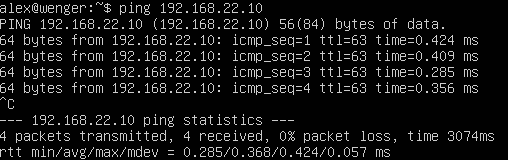
\includegraphics[scale=0.8]{resources/2-4-1.png}\\
Ping PC2 Router from PC1\\~\\
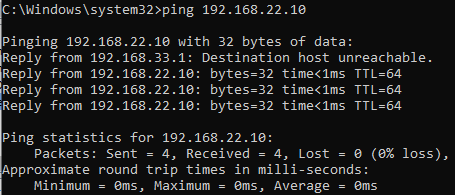
\includegraphics[scale=0.8]{resources/2-4-2.png}\\
Ping PC2 from PC Host\\~\\
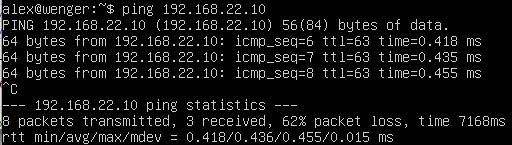
\includegraphics[scale=0.8]{resources/2-4-3.png}\\
Ping PC2 from Server
\end{center}

\section{DHCP Server}
This first screenshot shows that all DHCP servers have been disabled in the VB interface manager.\\

\textbf{5.} First, edit the file /etc/default/isc-dhcp-server with root permissions:
\begin{verbatim}
INTERFACES="enp0s8 enp0s9"
\end{verbatim}
The following entry defines the LAN and the router of the LAN. The IP-addresses 192.168.1.1 to 192.168.1.255 are typical for an intranet. Here only the range 192.168.1.1 to 192.168.1.254 are permitted.
\begin{verbatim}
subnet 192.168.1.0 netmask 255.255.255.0 {
  range 192.168.1.1 192.168.1.254;
  option routers 192.168.1.1;
}
\end{verbatim}
Attribute manually the first available address on each subnet to the gateway.
\begin{center}
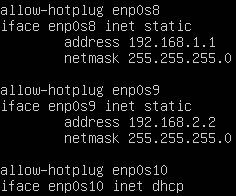
\includegraphics[scale=0.8]{resources/3-1-2.png}\\
Contents of "/etc/network/interfaces"
\end{center}
To assign a fixed address to a particular machine add a statement like the following to the configuration file. The cryptic number 00:0D:87:B3:AE:A6 is the hardware address of the interface of Server.
\begin{verbatim}
host Server {
  hardware ethernet 00:0D:87:B3:AE:A6;
  fixed-address 192.168.1.2;
}
\end{verbatim}
\begin{center}
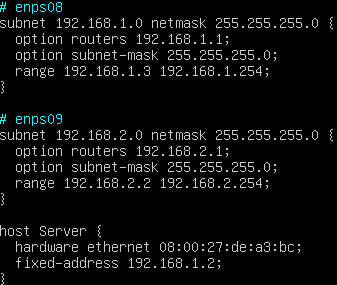
\includegraphics[scale=0.8]{resources/3-1-1.png}\\
Contents of "/etc/dhcp/dhcpd.conf"
\end{center}
To make all the changes effective, restart the DHCP daemon and reset the interfaces.
\begin{verbatim}
service isc-dhcp-server restart
sudo ifdown enp0s8
sudo ifup enp0s8
sudo ifdown enp0s9
sudo ifup enp0s9
\end{verbatim}
Here is the current IP configuration:
\begin{center}
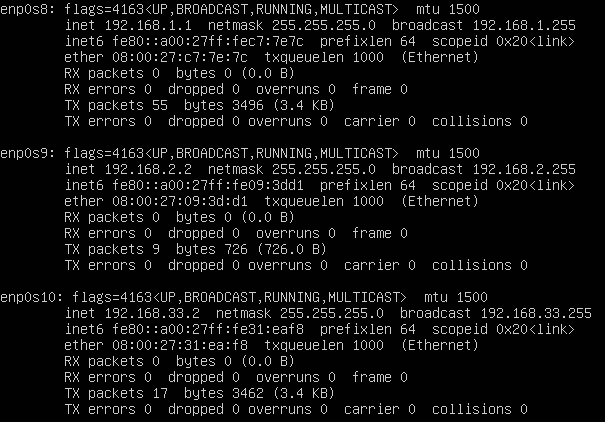
\includegraphics[scale=0.8]{resources/3-1-3.png}\\
PC Router\\~\\
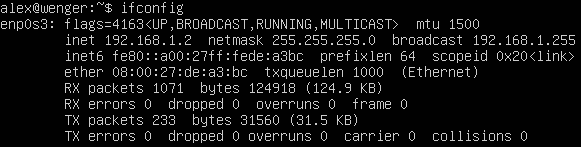
\includegraphics[scale=0.8]{resources/3-2-1.png}\\
Server
\end{center}
Now let's test pinging on PC1 from PC2.
\begin{center}
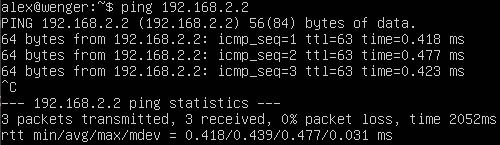
\includegraphics[scale=0.8]{resources/3-3-1.png}\\
PC1 to PC2\\~\\
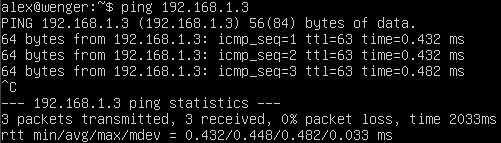
\includegraphics[scale=0.8]{resources/3-3-2.png}\\
PC2 to PC1
\end{center}

\section{HTTP Server}
\textbf{8.} Instead of using \texttt{ssh}, we will be using \texttt{scp} which is a means of securely transferring computer files between a local host and a remote host or between two remote hosts. It is based on the Secure Shell (SSH) protocol.
\begin{verbatim}
scp alex@192.168.33.1:index.html /var/www/html
\end{verbatim}
Now we need to reset the apache2 server.
\begin{verbatim}
service apache2 reload
\end{verbatim}
Next, open a web browser and type \texttt{192.168.1.2/index.html}. We get the following web page.
\begin{center}

\includegraphics[scale=0.8]{resources/4-1-1.png}
\end{center}

\textbf{9.} Capture with Wireshark an HTTP traffic on PC-Host.
\begin{center}
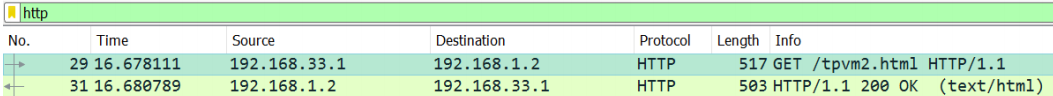
\includegraphics[scale=0.5]{resources/4-2-1.png}
\end{center}
HTTP provides a general framework for access control and authentication. The most common HTTP authentication is based on the "Basic" schema. The screenshot below shows an introduction to the HTTP framework for request and reply as well as authentication.
\begin{center}
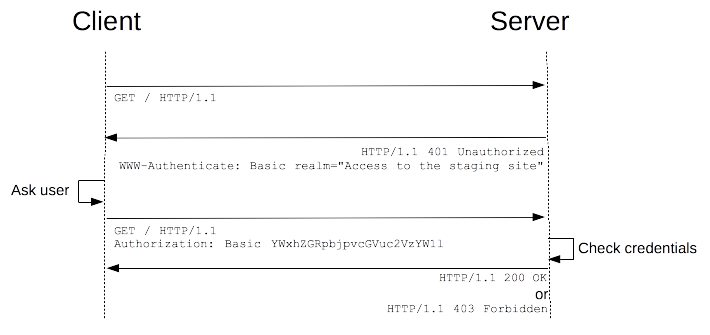
\includegraphics[scale=0.8]{resources/4-2-2.png}\\
Basic authentication HTTP protocol
\end{center}

\section{FTP Server}
\subsection{TCP Understanding}
In this section, we have to change the IP configuration of the lab. At ECE School, the private network is of the form 10.X.X.X whereas my home network has 192.168.1.X. Therefore, we'll simplify the network.\\

We want to filter out the file transfer traffic, therefore we show only the TCP traffic in Wireshark. To connect to the machine, use:
\begin{verbatim}
ftp <machine-ip-address>
\end{verbatim}
At times we wish to copy files from a remote machine using anonymous FTP. When the remote machine asks for a login, type in the word \texttt{anonymous}.
\begin{center}
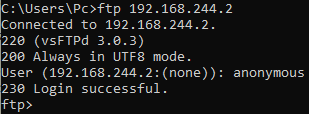
\includegraphics[scale=0.8]{resources/5-1-1.png}\\
Anonymous login on the FTP Server
\end{center}
On the following screenshot, we can clearly see the connection process. On line 306, we sent a request for the user \texttt{anonymous} which was accepted on line 307.
\begin{center}
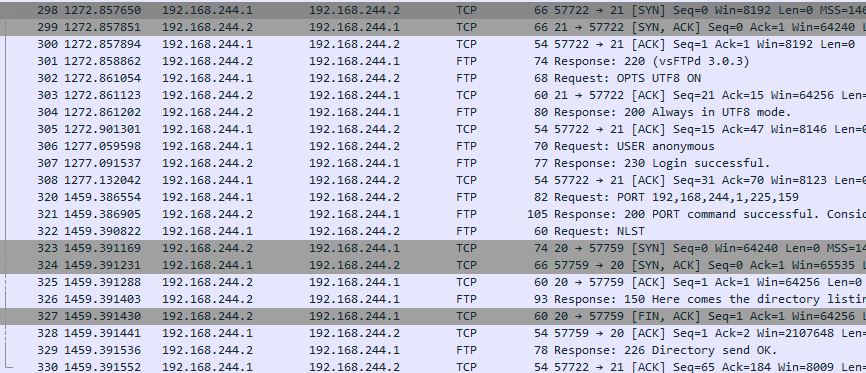
\includegraphics[scale=0.6]{resources/5-1-2.png}
\end{center}
Now let's test the \texttt{ls -l} command and capture the traffic.
\begin{center}
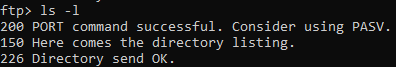
\includegraphics[scale=0.8]{resources/5-1-3.png}
\end{center}
Line 351 shows the requested command. After that, we receive the directory listing as displayed on line 355.
\begin{center}
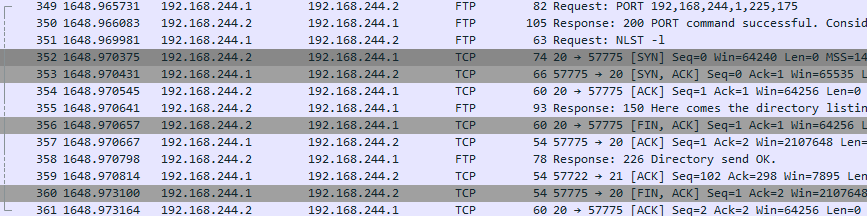
\includegraphics[scale=0.6]{resources/5-1-4.png}
\end{center}
Next, we send the file to the server.
\begin{verbatim}
put <file>
\end{verbatim}
\begin{center}
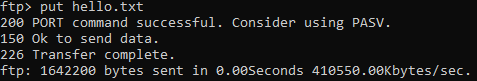
\includegraphics[scale=0.8]{resources/5-2-2.png}
\end{center}
Let's take a look at the corresponding traffic.
\begin{center}
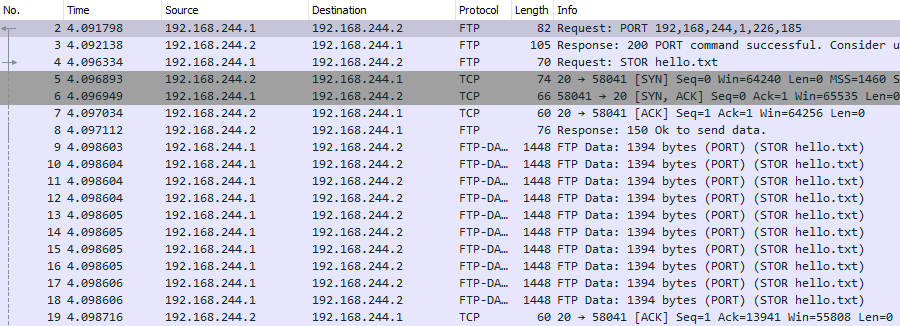
\includegraphics[scale=0.6]{resources/5-2-1.png}
\end{center}
The figure above corresponds to the first 19 frames of the exchange between the host and the remote FTP server.\\

\textbf{10.} Identify the connection establishment and connection release of this file transfer.
\begin{center}
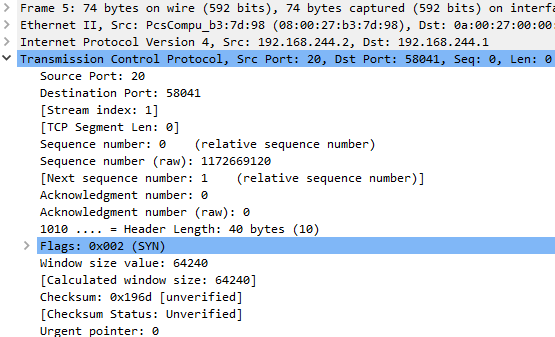
\includegraphics[scale=0.8]{resources/5-3-1.png}
\end{center}
We analyze the packet establishing the connection down after. Let's explore the flags.
\begin{verbatim}
Flags: 0x002 (SYN)
    000. .... .... = Reserved: Not set
    ...0 .... .... = Nonce: Not set
    .... 0... .... = Congestion Window Reduced (CWR): Not set
    .... .0.. .... = ECN-Echo: Not set
    .... ..0. .... = Urgent: Not set
    .... ...0 .... = Acknowledgment: Not set
    .... .... 0... = Push: Not set
    .... .... .0.. = Reset: Not set
    .... .... ..1. = Syn: Set
    .... .... ...0 = Fin: Not set
\end{verbatim}
The SYN flag synchronizes sequence numbers to initiate a TCP connection.
\begin{verbatim}
Ethernet II, Src: PcsCompu_b3:7d:98 (08:00:27:b3:7d:98),
             Dst: 0a:00:27:00:00:0c (0a:00:27:00:00:0c)
    Destination: 0a:00:27:00:00:0c (0a:00:27:00:00:0c)
    Source: PcsCompu_b3:7d:98 (08:00:27:b3:7d:98)
    Type: IPv4 (0x0800)
\end{verbatim}
The source MAC address corresponds to the MAC address of the FTP server as can be seen on the screenshot below.
\begin{center}
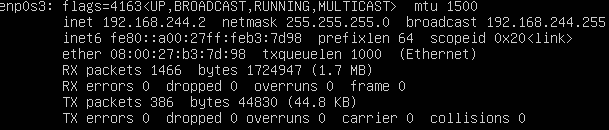
\includegraphics[scale=0.8]{resources/5-3-3.png}
\end{center}
The destination MAC address corresponds to the virtual interface of the VirtualBox Host-Only Adapter.
\begin{center}
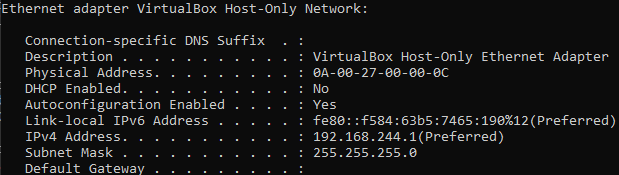
\includegraphics[scale=0.8]{resources/5-3-2.png}
\end{center}
The figure below describes the TCP connection establishment.
\begin{center}
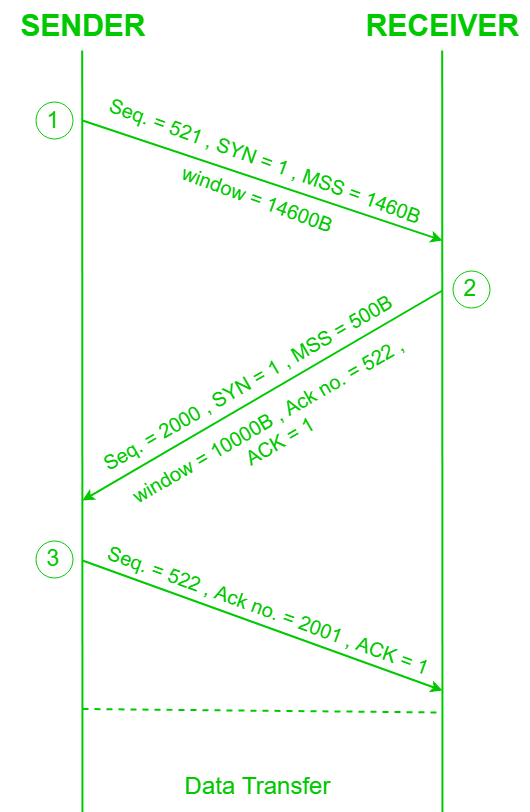
\includegraphics[scale=0.8]{resources/5-3-4.png}
\end{center}
Now let's take a look at the closing packet.
\begin{center}
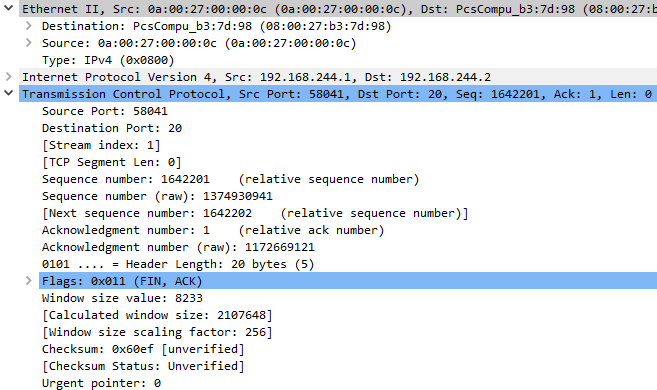
\includegraphics[scale=0.6]{resources/5-3-5.png}
\end{center}
\begin{verbatim}
Flags: 0x011 (FIN, ACK)
    000. .... .... = Reserved: Not set
    ...0 .... .... = Nonce: Not set
    .... 0... .... = Congestion Window Reduced (CWR): Not set
    .... .0.. .... = ECN-Echo: Not set
    .... ..0. .... = Urgent: Not set
    .... ...1 .... = Acknowledgment: Set
    .... .... 0... = Push: Not set
    .... .... .0.. = Reset: Not set
    .... .... ..0. = Syn: Not set
    .... .... ...1 = Fin: Set
\end{verbatim}
The FIN flag indicates the end of data transmission to finish a TCP connection. This frame is also and acknowledgment.
\begin{verbatim}
Ethernet II, Src: 0a:00:27:00:00:0c (0a:00:27:00:00:0c),
             Dst: PcsCompu_b3:7d:98 (08:00:27:b3:7d:98)
    Destination: PcsCompu_b3:7d:98 (08:00:27:b3:7d:98)
    Source: 0a:00:27:00:00:0c (0a:00:27:00:00:0c)
    Type: IPv4 (0x0800)
\end{verbatim}
The figure below describes the TCP connection termination.
\begin{center}
\includegraphics[scale=0.7]{resources/5-3-6.png}
\end{center}

\textbf{11.} Here are the 10 first data segments.
\begin{center}
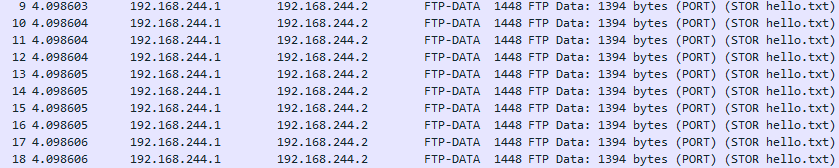
\includegraphics[scale=0.6]{resources/5-4-1.png}
\end{center}
Here are the first two packets.
\begin{verbatim}
Transmission Control Protocol, Src Port: 58041, Dst Port: 20,
                               Seq: 1, Ack: 1, Len: 1394
    Source Port: 58041
    Destination Port: 20
    [Stream index: 1]
    [TCP Segment Len: 1394]
    Sequence number: 1    (relative sequence number)
    Sequence number (raw): 1373288741
    [Next sequence number: 1395    (relative sequence number)]
    Acknowledgment number: 1    (relative ack number)
    Acknowledgment number (raw): 1172669121
    0101 .... = Header Length: 20 bytes (5)
    Flags: 0x010 (ACK)
        000. .... .... = Reserved: Not set
        ...0 .... .... = Nonce: Not set
        .... 0... .... = Congestion Window Reduced (CWR): Not set
        .... .0.. .... = ECN-Echo: Not set
        .... ..0. .... = Urgent: Not set
        .... ...1 .... = Acknowledgment: Set
        .... .... 0... = Push: Not set
        .... .... .0.. = Reset: Not set
        .... .... ..0. = Syn: Not set
        .... .... ...0 = Fin: Not set
        [TCP Flags: ·······A····]
    Window size value: 8233
    [Calculated window size: 2107648]
    [Window size scaling factor: 256]
    Checksum: 0x5e93 [unverified]
    [Checksum Status: Unverified]
    Urgent pointer: 0
    [SEQ/ACK analysis]
        [iRTT: 0.000141000 seconds]
        [Bytes in flight: 1394]
        [Bytes sent since last PSH flag: 1394]
    [Timestamps]
    TCP payload (1394 bytes)
\end{verbatim}
\begin{verbatim}
Transmission Control Protocol, Src Port: 58041, Dst Port: 20,
                               Seq: 1395, Ack: 1, Len: 1394
    Source Port: 58041
    Destination Port: 20
    [Stream index: 1]
    [TCP Segment Len: 1394]
    Sequence number: 1395    (relative sequence number)
    Sequence number (raw): 1373290135
    [Next sequence number: 2789    (relative sequence number)]
    Acknowledgment number: 1    (relative ack number)
    Acknowledgment number (raw): 1172669121
    0101 .... = Header Length: 20 bytes (5)
    Flags: 0x010 (ACK)
        000. .... .... = Reserved: Not set
        ...0 .... .... = Nonce: Not set
        .... 0... .... = Congestion Window Reduced (CWR): Not set
        .... .0.. .... = ECN-Echo: Not set
        .... ..0. .... = Urgent: Not set
        .... ...1 .... = Acknowledgment: Set
        .... .... 0... = Push: Not set
        .... .... .0.. = Reset: Not set
        .... .... ..0. = Syn: Not set
        .... .... ...0 = Fin: Not set
        [TCP Flags: ·······A····]
    Window size value: 8233
    [Calculated window size: 2107648]
    [Window size scaling factor: 256]
    Checksum: 0xeb23 [unverified]
    [Checksum Status: Unverified]
    Urgent pointer: 0
    [SEQ/ACK analysis]
        [iRTT: 0.000141000 seconds]
        [Bytes in flight: 2788]
        [Bytes sent since last PSH flag: 2788]
    [Timestamps]
    TCP payload (1394 bytes)
\end{verbatim}
The size of the payload is 1394 bytes. The sequence number starts with 1 and increases by 1394 bytes at every packet sent. That's why we have 1, 1395, 2789, etc. as sequence number.\\

\textbf{12.} Identify the segments that acknowledge the reception of these segments.
\begin{center}
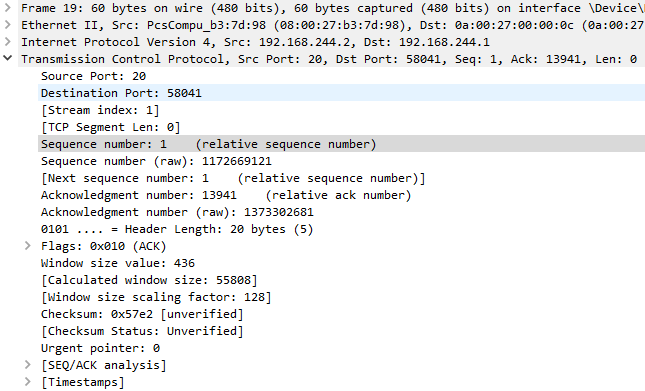
\includegraphics[scale=0.8]{resources/5-5-1.png}
\end{center}
This frame is an acknowledgment for the 10 first packets.\\

\textbf{13.} There is no re-transmission of any frame. This would be seen if we had a frame with the same sequence number.\\

\textbf{14.} Study and analyze the impact of the receiver's buffer space on the sender (based on window size advertisement). Display the window scaling graph.
\begin{center}
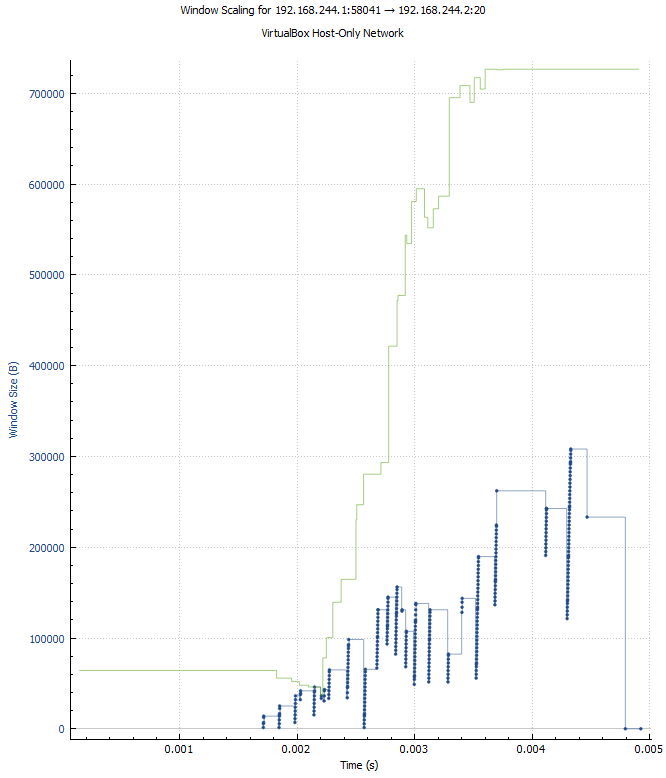
\includegraphics[scale=0.7]{resources/5-6-1.png}
\end{center}

\textbf{15.} Display throughput graphs in both connection directions.
\begin{center}
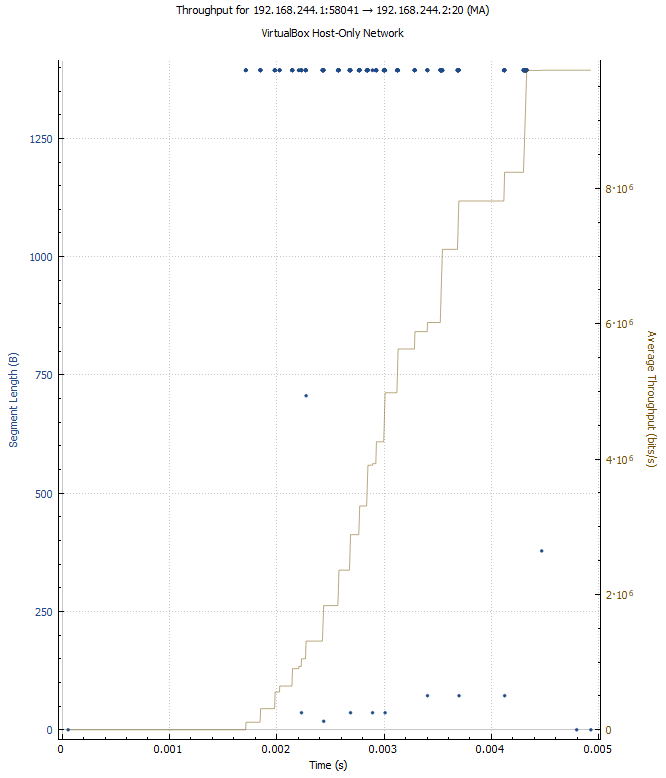
\includegraphics[scale=0.7]{resources/5-6-2.png}
\end{center}
\begin{center}
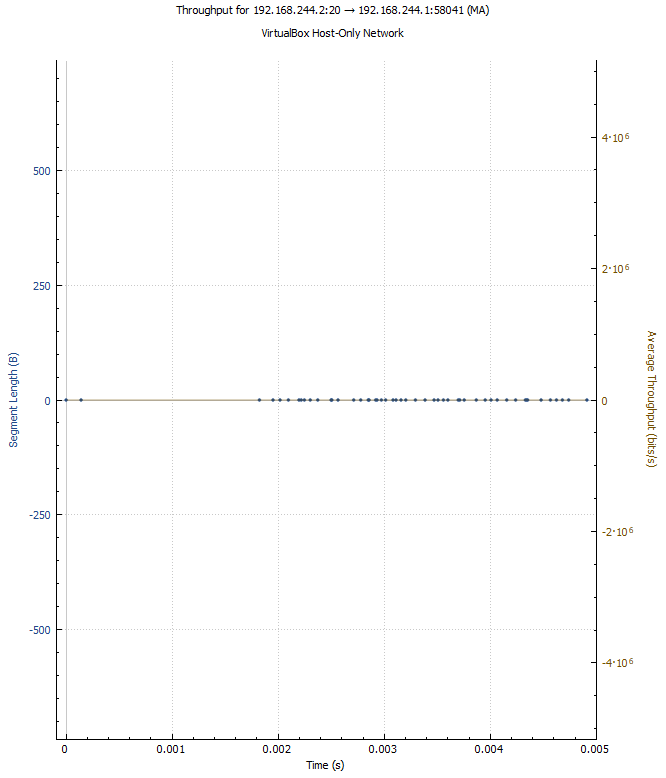
\includegraphics[scale=0.7]{resources/5-6-3.png}
\end{center}

\subsection{FTP Understanding}
\begin{center}
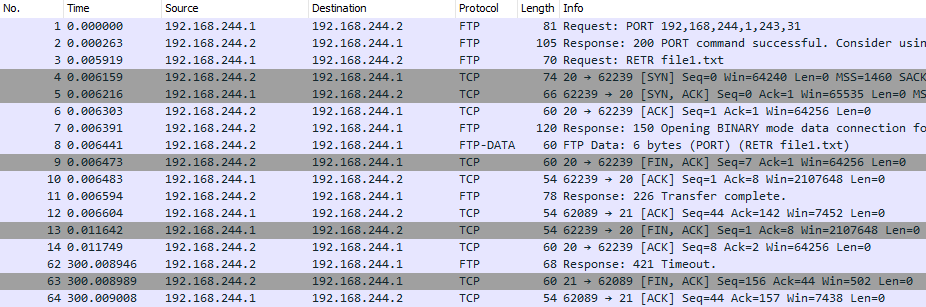
\includegraphics[scale=0.6]{resources/6-1-1.png}
\end{center}

\end{document}
